\chapter{Resultados e Discussão}

Este capítulo é destinado à exposição dos resultados do sistema de classificação de tipografias, contendo a análise e discussão destes no caso da utilização dos dois diferentes modelos classificadores, SVM e \textit{Random Forest}.

\section{Classificação das Tipografias}

O sistema desenvolvido deve receber uma imagem e indicar a qual tipografia o caractere presente na imagem pertence, dentre aquelas escolhidas para compor o projeto. Sendo assim, as possíveis classes para as imagens são:

\begin{enumerate}
\item Adobe Jenson
\item Adobe Garamond
\item Baskerville
\item Didot
\item Clarendon Bold
\item Franklin Gothic URW Demi
\item Helvetica
\item Futura Book
\item Gill Sans
\end{enumerate}

Como descrito no capítulo anterior, o resultado da classificação das tipografias foi mensurado a partir de testes de predição utilizando validação cruzada e computando sua acurácia variadas vezes. Além disso, o sistema foi sendo desenvolvido com o banco de imagens sendo incrementado de tipografia a tipografia e, em cada passo, realizada a validação cruzada e os testes de predição, bem como calculada a acurácia desse estágio. Todos esses dados são explicitados nas seções a seguir.

\subsection{Utilizando Support Vector Machine}

Primeiramente, utilizou-se para extração de atributos o modelo LBP e, para o classificador, o modelo linear SVM. Na tabela \ref{tab:svmResults} pode-se verificar o resultado de acurácia obtido mediante a utilização de banco de imagens de diferentes versões. As tipografias presentes em cada banco de imagens são apresentadas na tabela, iniciando-se somente com \textit{Helvetica} e \textit{Garamond} e prosseguindo a incrementação do banco de imagens, tipografia à tipografia. Além disso, o leitor pode acompanhar na Figura \ref{fig:graficoSVM} o histórico da acurácia do sistema classificador utilizando os modelos citados.

%%% Tabela

\begin{table}[h]
 \centering
 \begin{tabular}{l|c|c|c|c|c|c|c|c|c|c}
    Quantidade de tipografias  & 2 & 3 & 4 & 5 & 6 & 7 & 8 & 9\\ no banco de imagens & & & & & & & & \\
	\hline
	Helvetica & X & X & X & X & X & X & X & X   \\
	Garamond & X & X & X & X & X & X & X & X  \\
	Clarendon &  & X & X & X & X & X & X & X    \\
	Futura &  &  & X & X & X & X & X & X  \\
	Baskerville &  &  &  & X & X & X & X & X    \\
	Didot &  &  &  &  & X & X & X & X    \\
	Gill Sans &  &  &  &  &  & X & X & X   \\
	Jenson &  &  &  &  &  &  & X & X  \\
	Franklin Gothic &  &  &  &  &  &  &  & X  \\
	\hline
	Acurácia [\%] & 94,2 & 83,16 & 64,47 & 57,58 & 55,94 & 50,44 & 48,15 & 45,53 \\
	Desvio padrão [\%] & 2 & 5 & 4 & 5 & 2 & 2 & 3 & 3\\
 \end{tabular}
 \caption{Resultados de acurácia em testes de validação cruzada do sistema classificador utilizando o modelo SVM, avaliado com banco de imagens em processo de incrementação tipografia à tipografia - \textbf{Fonte:} Autora}
 \label{tab:svmResults}
\end{table}

%%% gráfico

\begin{figure}[H]
 \centering
  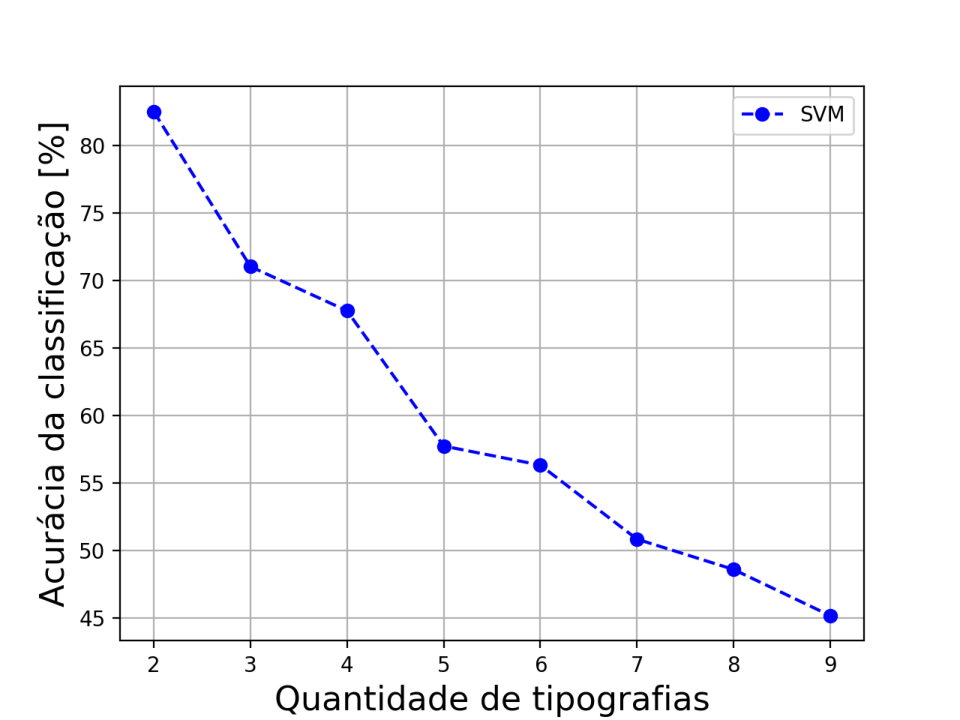
\includegraphics[width=0.7\linewidth]{figuras/graficosvm.pdf}
  \caption{Gráfico do desempenho do sistema classificador com o modelo SVM em relação à quantidade de tipografias presentes no banco de imagens - \textbf{Fonte:} Autora}
  \label{fig:graficoSVM}
\end{figure}

Percebe-se que, a cada incremento no banco de imagens, a acurácia é bastante comprometida, chegando ao baixo índice de 45,53\%, desvio padrão de 3\%, com banco de imagens completo. Diante do nível de acurácia bastante insatisfatório em comparação com trabalhos similares com índices de 85\% e 96,91\%, decidiu-se aplicar outro modelo classificador \citeC{la1999} \citeC{zramdini1998}. O resultado ruim pode ser fruto de uma sensibilidade do modelo SVM quanto aos atributos (dados) que lhe são fornecidos durante a etapa de treinamento \citeC{lorena2007}. Além disso, como já comentado anteriormente, a classificação é dificultada diante do alto grau de similaridade entre algumas tipografias presentes no projeto.

Portanto, para continuar empregando o classificador SVM, um modelo mais robusto de extração de atributos deveria ser utilizado, o que seria também uma opção para implementação do sistema. Porém, optou-se por manter o LBP para extração de atributos devido ao seu baixo custo computacional e rapidez de execução, critério importante no cenário de grande volume de dados e também por ser uma aplicação interativa, em se tratando de um produto final.

É ainda importante enfatizar a influência do conjunto de dados composto para o treinamento e testes no caso de aprendizado de máquina. Como descrito no capítulo anterior, o primeiro banco de imagens criado para treinamento e testes do sistema classificador comprometeu severamente a acurácia da classificação realizada pelo sistema. A Tabela X apresenta uma comparação entre os resultados obtidos com o banco de imagens precedente e o banco de imagens após maior refinamento.

\subsection{Utilizando Random Forest Classifier}

O segundo classificador utilizado foi o \textit{Random Forest Classifier}, ainda com o modelo LBP para extração de atributos das imagens. Assim como na primeira versão do sistema, o modelo classificador foi treinado com oito versões do banco de imagens. A primeira versão é composta de duas tipografias que são suficientemente distintas entre si e então, a cada versão, o banco de imagens é incrementado com um conjunto de imagens de uma das tipografia presentes no projeto. Os resultados de acurácia da classificação performada pelo sistema utilizando \textit{Random Forest} como classificador são expostos na Tabela \ref{tab:rfcResults} e, na Figura \ref{fig:grafico2}, pode-se ver a comparação dos resultados do classificador SVM e do classificador \textit{Random Forest} a medida em que o banco de imagens foi sendo incrementado.


%%% Tabela

\begin{table}[h]
 \centering
 \begin{tabular}{l|c|c|c|c|c|c|c|c|c|c}
    Quantidade de tipografias  & 2 & 3 & 4 & 5 & 6 & 7 & 8 & 9\\ no banco de imagens & & & & & & & & \\
	\hline
	Helvetica & X & X & X & X & X & X & X & X   \\
	Garamond & X & X & X & X & X & X & X & X  \\
	Clarendon &  & X & X & X & X & X & X & X    \\
	Futura &  &  & X & X & X & X & X & X  \\
	Baskerville &  &  &  & X & X & X & X & X    \\
	Didot &  &  &  &  & X & X & X & X    \\
	Gill Sans &  &  &  &  &  & X & X & X   \\
	Jenson &  &  &  &  &  &  & X & X  \\
	Franklin Gothic &  &  &  &  &  &  &  & X  \\
	\hline
	Acurácia [\%] & 99,27 & 95,38 & 91,54 & 87,82 & 87,96 & 85,09 & 85,03 & 84,87 \\
	Desvio padrão [\%] & 0 & 2 & 1 & 3 & 2 & 3 & 2 & 3\\
 \end{tabular}
 \caption{Resultados de acurácia em testes de validação cruzada do sistema com o modelo Random Forest, avaliado com banco de imagens em processo de incrementação tipografia à tipografia - \textbf{Fonte:} Autora}
 \label{tab:rfcResults}
\end{table}


%%% gráfico

\begin{figure}[H]
 \centering
  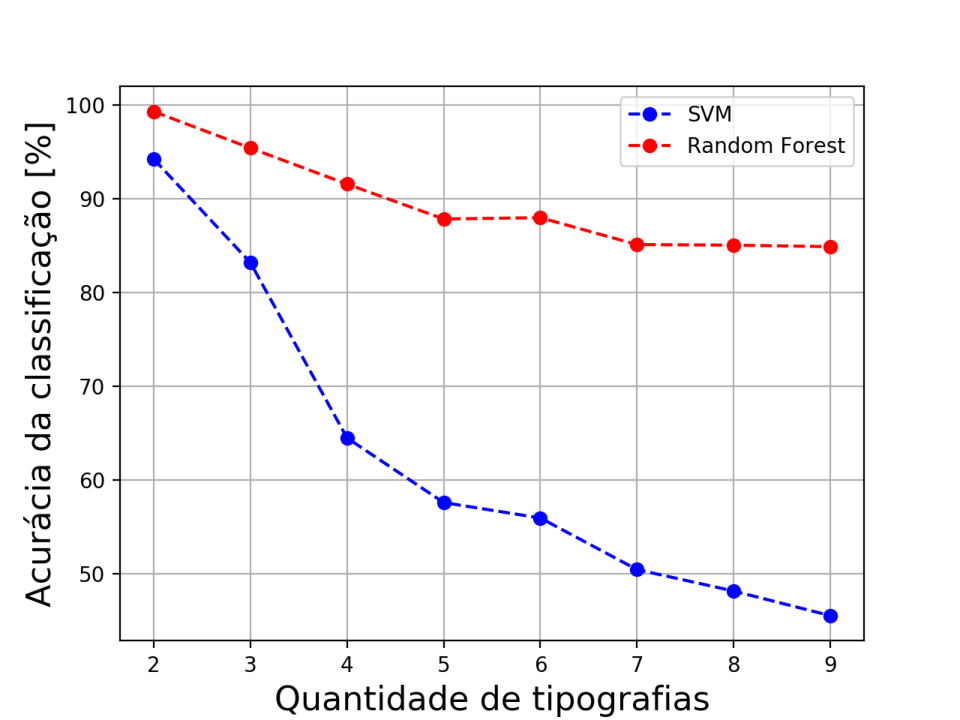
\includegraphics[width=0.7\linewidth]{figuras/graficosvmrfc.pdf}
  \caption{Gráfico do desempenho do sistema classificador com os dois modelos utilizados, SVM e \textit{Random Forest}, em relação à quantidade de tipografias presentes no banco de imagens - \textbf{Fonte:} Autora}
  \label{fig:grafico2}
\end{figure}

Sendo assim, o resultado final obtido para a classificação das nove tipografias apresentou uma acurácia de 84,87\%, com desvio padrão de 3\%. O desempenho encontrado foi bastante superior ao caso anterior devido à alteração do modelo, elevando a acurácia do sistema classificador a um valor satisfatório. Apesar de ainda ser passível de melhoria, o desempenho foi similar ao encontrado em trabalho semelhante, que apresentou acurácia de 85\%, portanto, suficiente para um primeiro estágio no momento \citeC{la1999}.

Nota-se a grande discrepância entre o desempenho do sistema empregando o classificador \textit{Random Forest} e o SVM. Esse resultado pode ser derivado de vários aspectos, entre eles, o perfil do conjunto de dados necessário para garantir um bom funcionamento do SVM como classificador.

O SVM com \textit{kernel} linear foi aquele que obteve melhor resultado apesar de vários treinamentos da máquina terem sido efetuados com outras opções de \textit{kernel}, que podem ser vistos na Tabela \ref{tab:svmkernelResults}. Implementações com modelos não-lineares foram realizados somente no estágio final do banco de imagens, ou seja, com conjunto completo de nove tipografias.

\begin{table}[h]
 \centering
 \begin{tabular}{l|c|c}
    Kernel & Acurácia [\%] & Desvio Padrão [\%]\\
	\hline
	Linear &  45,53 & 3 \\
	RBF & 37,28 & 4 \\
	Polinomial & 18,01 & 6  \\
	Sigmoid & 35,61 & 5 \\
 \end{tabular}
 \caption{Resultados de acurácia em testes de validação cruzada do sistema com o modelo SVM avaliado com diferentes \textit{kernels} em banco de imagens completo - \textbf{Fonte:} Autora}
 \label{tab:svmkernelResults}
\end{table}

Vale notar que o SVM linear obtém bom desempenho como classificador em conjuntos de dados com distribuição linear, ou que se aproximem desse padrão. Já no caso da utilização de \textit{kernel} não-linear, o conjunto de treinamento é mapeado para um espaço com dimensão superior e que seja mais suscetível à uma separação linear das classes \citeC{lorena2007}.

No entanto, os dois casos possuem um grau de dependência da distribuição do conjunto original de dados para que apresentem bom desempenho na classificação. Além disso, como pode-se perceber por sua característica linear intrínseca, o modelo SVM foi concebido como um classificador binário e, posteriormente, adaptado para conjuntos não-lineares em casos de multi-classificação \citeC{boser1992}. Dessa forma, a utilização do SVM nesse caso depende de uma série de parâmetros que devem ser bem ajustados para que ocorra a separação linear de forma ótima, o que dificulta sua utilização, fator que pode ter sido decisivo em seu desempenho neste projeto.

Em relação ao modelo classificador \textit{Random Forest}, os motivos pelos quais sua aplicação resultou em desempenho satisfatório podem estar relacionados à robustez do modelo em relação à distribuição e características gerais do conjunto de dados de entrada na máquina, já que, para seu bom funcionamento, não depende da linearidade da distribuição dos dados. Além disso, por se tratar de um modelo construído, em sua maioria, por árvores de decisão (\textit{decision trees}), possui uma capacidade ampliada para lidar com espaços de variadas dimensões e também com um número alto de amostras de treinamento. Sendo assim, o \textit{Random Forest} pode ser considerado como um modelo que é intrinsicamente ajustado para multi-classificação, fato que facilita a sua utilização no caso aqui apresentado.

%As SVMs lineares são eficazes na classificação de conjuntos de dados linearmente se- paráveis ou que possuam uma distribuição aproximadamente linear, sendo que a versão de margens suaves tolera a presença de alguns ruídos e outliers. Porém, há muitos casos em que não é possível dividir satisfatoriamente os dados de treinamento por um hiperplano. Um exemplo é apresentado na Figura 8a, em que o uso de uma fronteira curva seria mais adequada na separação das classes. \citeC{lorena2007}

%As SVMs lidam com problemas não lineares mapeando o conjunto de treinamento de seu espaço original, referenciado como de entradas, para um novo espaço de maior dimensão, denominado espaço de características (feature space) [15]. Seja Φ : X → I um mapeamento, em que X é o espaço de entradas e I denota o espaço de características. A escolha apropriada de Φ faz com que o conjunto de treinamento mapeado em I possa ser separado por uma SVM linear. (BOA FIGURA NO ARTIGO)
